\chapter{Background}
\label{chap:background}
This chapter gives a general introduction into the vocabulary of financial computing and the machine learning techniques employed.

\section{Trading Basics}
In order to understand the objective of this thesis, fundamental knowledge about the domain of financial computing is obligatory. This chapter provides a quick overview.

\subsection{Financial Instruments}
Financial instruments represent legal agreements of monetary value between parties and can be traded as assets. These assets span from  actual cash, through evidence of entity or share ownership, to contractual rights to receive or deliver another type of financial instrument.

\subsection{Markets}
Financial instruments are typically traded through one of two basic market types:
\begin{description}
\item[Over-The-Counter (OTC)] In an OTC or off-exchange market, transactions take place directly between two parties, without a mediator. Prices are negotiated directly between buyer and seller and typically not published to the public.
\item[Exchange] In exchange markets, transactions are executed by a so called broker. A broker, which can be both, an individual or a firm, executes buy and sell orders on behalf of traders for a certain fee or commission. The respective prices are determined by the current market situation, in particular by supply and demand.
\end{description}

\subsection{Exchange Markets}

Specialized exchanges concentrate on certain sub-types of financial instruments and offer a trading venue for those willing to buy and sell these instruments. Some of them are listed below:
 
\begin{description}
\item[Stock Exchange Market] A stock exchange or bourse provides companies access to investment capital in exchange to a share of ownership. Especially in times with notoriously low interest rates, investors tend to accept the greater risk of business development over a risk free, but faint investment, to grow their assets.\\
\Eg \acs{NASDAQ}, Deutsche B�rse, \dots{}
\item[Commodity exchange market] Commodity exchange markets allow for speculations with goods like oil, gold, corn, \dots{} \\
\Eg \acs{Eurex}, \dots{}
\item[Foreign exchange market] Foreign exchange (short: forex) is considered the largest financial market in the world. The forex market is responsible for determining currency exchange rates.\\
\Eg FXCM, \dots{}
\item[Digital assets exchange market] Digital asset exchange markets allow for speculations with virtual goods, like digital documents, motion picture, audible content, or digital currencies (\ie electronic money).\\
\Eg Poloniex, \dots{}
\end{description}

In the past, exchanges were physical locations. In many cases, these physical locations have been replaced by fully electronically organized markets, accessible through the internet. As a result, more traders can execute orders in a higher frequency.

\subsection{Ask and Bid}
Most exchange markets function after the so called auction market model \Cite{Klemperer99auctiontheory}, where the exchange acts as a mediator between buyers and sellers to ensure fair trading. Here buyers can \emph{bid} a price they are willing to pay for a certain number of shares and sellers can \emph{ask} a price they are aiming to make with a number of shares.
The highest of all bids is called the \emph{bid price}, the lowest of all offers is called the \emph{ask price}. Together they represent the current price at which an instrument is traded.\\

The difference between bid price and ask price is called \emph{bid-ask spread}, often abbreviated to \emph{spread}.

\subsection{Limit Order Book and Market Depth}
A limit orderbook reflects supply (asks) and demand (bids) for a particular financial instrument. It is usually maintained by the trading venue and lists the number of shares being bid or offered, organized by price levels in two opposing books. Incoming orders are constantly appended to this highly dynamic list, while a matching engine cautiously resolves any inconsistencies (\ie overlaps) between asks and bids by mediating between the involved parties.\\

It is usually not before the matching engine has arranged an actual trade, that a trading venue claims a certain percentage of the turnover as a service fee. To encourage active market participation, the pure submission, revision and cancelation of orders is typically free of charge.\\

\begin{table}
\centering
	\scalebox{0.6}{
\begin{tabular}{lrlrrr}
\toprule
{} &  Amount &    Type &  Volume &  VolumeAcc &  norm\_Price \\
\midrule
31.00 &   \color{mymauve}200.0 &     ask &  6200.0 &     8425.0 &    1.074533 \\
30.00 &    \color{mygreen}50.0 &     ask &  1500.0 &     2225.0 &    1.039871 \\
29.00 &    \color{red}25.0 &     ask &   725.0 &      725.0 &    1.005208 \\
28.85 &     NaN &  center &     NaN &        NaN &         NaN \\
28.70 &   200.0 &     bid &  5740.0 &     5740.0 &    0.994810 \\
28.50 &   100.0 &     bid &  2850.0 &     8590.0 &    0.987877 \\
28.00 &   300.0 &     bid &  8400.0 &    16990.0 &    0.970546 \\
\bottomrule
\end{tabular}}
\caption[Exemplary snapshot of a limit orderbook]{Exemplary snapshot of a limit orderbook for stocks of AIWC\protect\footnotemark.}
\label{table:orderbook:example}
\end{table}


\Cref{table:orderbook:example} shows a limit orderbook snapshot up to a market depth of 3, as seen by market participants. Here Alice offers {\color{red}25} shares per 29\$, Bob and Cedar offer {\color{mygreen}20 and 30} shares respectively per 30\$ and David offers {\color{mymauve}200} shares per 31\$\footnotetext{Acme Internet Widget Company}.\\


\label{sec:marketdata:levels}
Based on their trading needs, traders can typically choose between multiple levels of real-time market data.
\begin{description}
\item[Level 1 Market Data] Basic informations only:\\
Bid price + size, Ask price + size, Last price + size
\item[Level 2 Market Data] Additional access to the orderbook.\\
Usually data providers display the orderbook only up to a certain market depth $m$, \ie the lowest $m$ asks and the highest $m$ bids.
\item[Level 3 Market Data] Full data access.\\
Typically only accessible for the market maker.

\end{description}

\subsection{Slippage}
\label{chap:slippage}
Slippage is defined as the difference between expected and achieved price at which a trade is executed. Slippage may occur due to delayed trade execution. Especially during periods of high volatility, markets might change faster than the order takes to be executed. Slippage is also linked to the order size, as larger orders tend to \emph{eat} into the opposing book and are fulfilled at successively worse price levels. Slippage can be both positive or negative, depending on the current market movements and must be taken into account by serious investors.


\subsection{Order Types}
\label{chap:ordertypes}
Investors can execute orders of different types, of which the most common ones are described below:

\begin{description}
\item[Market Orders] are the most simple form of orders. Here, the investor only specifies the number of shares he want's to buy/sell and the full order is executed immediately, at any price. Especially for large-scale traders or traders with level 1 data access only, these simple market orders are rather hazardous, since the achieved price can significantly differ from the expected price due to sparse supply and demand.

\item[Limit Orders] additionally feature a worst price, \ie the highest price a buyer is willing to pay per share or respectively the lowest price a seller is willing to make per share. Limit orders are immediately placed into the orderbook and (partially) executed, once the matching engine finds a corresponding trade in the opposing book.\\
Limit orders reduce the risk of slippage, but do not guarantee execution.

\item[Hidden Orders] are placed into the market makers internal orderbook, but not displayed to other market participants with level 2 market data access. They represent a simple solution to large-scale investors seeking anonymity in the market, aiming to obfuscate their trading intention from other market participants.

\end{description}

\subsection{Trading strategies}
\label{chap:tradingstrategies}
An order placement typically originates from a carefully considered \emph{trading strategy}. An \emph{active} trading strategy buys and sells instruments frequently based on short-term price movements, whereas a \emph{passive} trading strategy such as \emph{Buy-And-Hold} believes in long-term price movements eventually outweighting any short-term fluctuations.\\

As the execution of trades typically implies trading costs and slippage, these have to be taken into account. Particularly active traders with a high order quantity and large-scale investors with high order volumes are concerned with this burden. The order type chosen has a major impact on speed of execution and slippage generated.\\

While \emph{limit orders} reduce the risk of slippage, they do not guarantee full order execution. This leads to the important problem of \emph{optimized trade execution}, which frequently occurs in the domain of financial computing. In its simplest form, the problem is defined by a particular financial instrument (here: Bitcoins), which must be bought or sold within a fixed time horizon, for the best achievable share price.\\

In \cite{Nevmyvaka2005SubmitAndLeave} Nevmyvaka \etal introduce a \ac{SL}, which cleverly combines market and limit orders: After an initial limit order submission, the order is left on the market for a predefined time horizon, after which it's unexecuted part is transformed into a market order and thus executed completely. They later extended their strategy to a \ac{SR} \cite{Nevmyvaka:2006}, where the order limit may be revised at discrete time steps, depending on trade progress and market changes.

%\subsection{Efficient Market Hypothesis}
%The \ac{EHM}, developed in 1970 by Eugene Fama\Cite{Fama70efficientcapital}, is an investment theory after that it is impossible to consistently \emph{beat the market} in exchange markets. According to this theory, financial instruments always trade at their fair price as new information are incorporated in real time, since all participants are inaugurated to the same information. Consequently, it should neither be possible for investors to earn above average returns from the overall market by purchasing undervalued shares or selling shares for inflated prices, nor to profit from proper market timing as addressed by the problem of \emph{optimized trade execution}.\\

%Later Malkiel showed empirically and theoretically\Cite{TheEfficentMarketHypothesisAndItsCritics} that the efficient market hypothesis is only valid under certain preconditions. While the paper concludes that most markets are very (not extremely!) efficient and that prices are far less predictable than some (at that time) recent academic papers claimed, there remains a certain degree at which asset prices are indeed predictable.\\


\section{Bitcoin}
\label{chap:bitcoins}
Bitcoin is a digital cryptocurrency, released in 2009 as open-source software under the name Satoshi Nakamoto \Cite{Davis:Bitcoin_inventor}. Motivated in part by anger over the foregone financial crisis, the underlying peer-to-peer system\Cite{Nakamoto_bitcoin:a}, provides a decentralized payment system. To this point, electronic transactions always required involving a third party to validate transactions, an inevitable necessity to forestall double-spending bitcoin tokens. Double-spending is a problem unique to digital currencies, as digital informations, in contrast to physical currencies, may be replicated arbitrarily. Rather than entrusting a central authority or central server with this validation task, a distributed public transaction log, known as the \emph{block chain}\Cite{Economist:Blockchain} is maintained among all participants.\\

The block chain is a continuously growing list of confirmed and timestamped transaction records, called \emph{blocks}. Every block includes a complex proof-of-work and a cryptographic hash of the previous block, making it extremely resistant against retrospective modifications. To motivate others to validate transactions, newly created bitcoins are rewarded to the first miner (or mining party), successfully serving the computationally demanding proof-of-work.\\

Through a manifold of legal and black markets, bitcoins may be exchanged for other currencies, products and services. In contrast to traditional exchanges, no regular trading hours exist. Transactions can be executed at all times, mostly unregulated and pseudonymous\footnote{Owners of bitcoin tokens are not explicitly identified, but bitcoin exchanges may collect personal data on their customers if required by law.}\Cite{WashingtonPost:Bitcoinfacts}. As a consequence, Bitcoin are particularly sensitive to extraordinary events or news, frequently causing immediate (panic) reactions. This effect is possibly leveraged by relatively low entry barriers, attracting amateur and professional traders likewise.

\subsection{Volatility}
\label{chap:bitcoin:volatility}
Bitcoin is a highly volatile currency, capable of massive price changes towards both directions within short periods of time. A high volatility provides profitable opportunities, but comes at the price of higher risk. Due to a very high trading volume\footnote{$\sim 40.000.000\$$ per 24h for currency pair BTC/USDT on Poloniex.\\Source: \url{https://coinmarketcap.com/exchanges/volume/24-hour} (accessed 12-July-2017)}, limit orderbooks are typically more condensed around the current best price than limit orderbooks of less frequently traded stocks. As a consequence, less slippage is to be expected from eating into the orderbook, while more slippages originates from general price fluctuations.\\

\Cref{fig:bitcoinvolatility} compares volatilities of currency pairs USDT/BTC (blue line) and USD/Pound (red line).

\begin{figure}[ht]
	\centering
	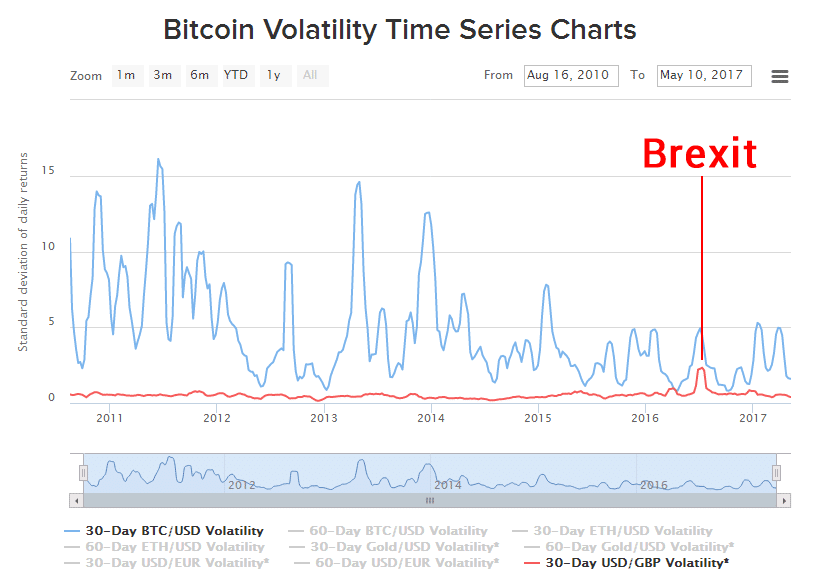
\includegraphics[width=0.6\textwidth]{content/images/BitcoinVolatility}
	\caption{BTC/USDT and USDT/Pound volatility compared.}
	\scriptsize Source: \url{https://99bitcoins.com/bitcoin-volatility-explained}
	\label{fig:bitcoinvolatility}
\end{figure}





\section{Supervised Learning}
Supervised learning is a subdomain of machine learning, where a function is learned from labeled training data $\{ (x_1, y_1), ..., (x_N, y_N) \} $. Each training sample maps a feature vector $x_i \in X$ to a desired target value or label $y_i \in Y$. Target values may either be categorial, making the learning task a \emph{classification} problem, or continuous, making the learning task a \emph{regression} problem.\\

A supervised learning algorithms seeks to find a general function $g_\theta()$ (or it's parameters $\theta$), such that $g_\theta(x_i) \approx y_i | i \leq N$. The learned function should ideally avoid overfitting by finding a generalization to previously unseen data.

{\color{red}Keep or Remove?! Or Move below \Cref{chap:RLfunctionapproximation}}

\subsection{Random Forest}
bla







\section{Reinforcement Learning}
\ac{RL} is a subdomain of machine learning. It was first defined by Sutton and Barto\Cite{Sutton98reinforcementlearning} as the problem of learning from interactions with an environment in order to achieve long-term goals. In contrast to \ac{SuL}, no labeled training data is present, such that sub-optimal actions can not be corrected explicitly. Instead, in each time step $t$, the agent takes the action $a_t$ which maximizes\footnote{Alternatively, it is possible to \emph{minimize} the future expected cost: $C_t = - R_t$} his future expected reward $R_t$, based on empirical knowledge.\\

\Cref{fig:rlagent} shows the typical \ac{RL} scenario. An agent (partially) observes a state $s_t$ and a reward $r_t$ at every discrete time step $t$. It takes an action $a_t$ and hereon receives a new state $s_{t+1}$ and reward $r_{t+1}$.\\


\tikzstyle{block} = [rectangle, draw, 
    text width=8em, text centered, rounded corners, minimum height=4em]
    
\tikzstyle{line} = [draw, -latex]

\begin{figure}[ht]
	\centering
\begin{tikzpicture}[node distance = 6em, auto, thick]
    \node [block] (Agent) {Agent};
    \node [block, below of=Agent] (Environment) {Environment};
    
     \path [line] (Agent.0) --++ (4em,0em) |- node [near start]{Action $a_t$} (Environment.0);
     \path [line] (Environment.190) --++ (-6em,0em) |- node [near start] {New state  $s_{t+1}$} (Agent.170);
     \path [line] (Environment.170) --++ (-4.25em,0em) |- node [near start, right] {Reward $r_{t+1}$} (Agent.190);
\end{tikzpicture}
	\caption{The discrete \ac{RL} scenario defined by Sutton and Barto\Cite{Sutton98reinforcementlearning}}
	\label{fig:rlagent}
\end{figure}

Rather than learning from labeled training data, the agent applies a \emph{trial and error} pattern and exploits (delayed) external rewards to find actions, maximizing the expected future reward. As actions may not necessarily show an immediate effect, rewards are often delayed and must be accounted for in the so called \emph{credit assignment problem}\Cite{MinskyManuscript-MINSTA}.\\

The expected future reward $R_t$ can be expressed by the cumulative reward of all successive rewards. The discounting factor $\gamma \in [0,1]$ represents the importance between long-term and short-term rewards. With a high $\gamma$, the agent aims to maximize long-term rewards, whereas a small $\gamma$ leads to greedy actions, favouring short-term rewards. 
\begin{equation}
	R_t = \sum_{i=0}^{\infty} \gamma^i r_{t+i+1}
\end{equation}







\subsection{Markov Decision Process}
In reinforcement learning, the environment is typically formulated as \ac{MDP} \Cite{Bel}, which provides a mathematical framework for optimization problems.\\

An \ac{MDP} is a discrete time stochastic control process, written as 5-tuple $(S, A, P, R, \gamma)$. It consists of a (finite) set of environment states $s \in S$, a (finite) set of actions $a_t \in A$, a transition probability matrix $P: S \times A \rightarrow \mathbb{P}(S)$, which maps from state-action pairs $(s_t, a_t)$ to a probability distribution over all successor states $s_{t+1} \in S$,
\begin{equation}
	P^a_{ss'} = \mathbb{P}[s_{t+1}=s' | s_t=s, a_t=a]
\end{equation}

and a reward (or cost) function $R: S \times A \rightarrow \mathbb{R}$, that computes the immediate reward received after applying action $a_t$ in state $s_t$.
\begin{equation}
	R^a_{s} = \mathbb{E}[r_{t+1} | s_t=s, a_t=a] = -\mathbb{E}[c_{t+1} | s_t=s, a_t=a]
\end{equation}

The discount factor $\gamma \in [0,1]$ eventually defines the level of foresightedness. It is obligatory in \ac{MDP}s with an infinite time horizon, to impede infinite values for accumulated long-term returns.\\

The general goal in reinforcement learning is to find optimal policies $\pi^*: S \rightarrow A$, that map states to the best applicable actions, such that the (discounted) expected long-term reward is maximized, or respectively the (discounted) expected long-term cost is minimized.
\begin{equation}
    \pi^*(s) = arg\max_{a \in A(s)} \mathbb{E}[R_t | s_t=s] \>=\> arg\min_{a \in A(s)} \mathbb{E}[C_t | s_t=s]
\end{equation}





\subsection{Markov Property}
An important condition of \ac{MDP}s is the \emph{Markov Property}, which defines the probability distribution of future states to be independent of the past ($s_{t-n}$), given the present ($s_t$). As such, states must capture all relevant information from the history, to deliver sufficient statistics of the future. A state $s_t$ is \emph{Markov} if and only if:
\begin{equation}
     \mathbb{P}(S_{t+1} = s' | s_t, a_t) = \mathbb{P}(s_{t+1} = s' | s_t, a_t, s_{t-1}, a_{t-1}, \ldots{})
\end{equation}






\subsection{Value Function and Bellmann Equation}
In order to find the optimal strategy $\pi^*$, the value of states and actions must be estimated. The state-value function $V^\pi: S \rightarrow \mathbb{R}$ returns the expected reward (or cost) when following $\pi$ from state $s$:
\begin{equation}\label{eq:valuefunction}
\begin{split}
     V^\pi(s) & = \mathbb{E}[R_t | s_t = s] \\
      & = \mathbb{E}_\pi [\sum_{k=0}^\infty \gamma^k r_{t+k+1} | s_t=s] \\
      & = \mathbb{E}_\pi [r_{t+1} + \gamma \sum_{k=1}^\infty \gamma\,^k r_{t+k+1} | s_t=s] \\
      & = \sum_{s' \in S} P(s' \,|\, s, \pi(s))\>[r(s, \pi(s), s') + \gamma\, V^\pi(s')]
\end{split}
\end{equation}

where $0 \leq \gamma \leq 1$ is the discount rate. Assuming an optimal policy $\pi^*$, the optimal value function may be rewritten as $V^{\pi^*} = V^*$ and Bellmann's \emph{principle of optimality} holds:

\begin{quote}
\emph{"An optimal policy has the property that whatever the initial state and initial decision are, the remaining decisions must constitute an optimal policy with regard to the state resulting from the first decision."}

\begin{flushright}
      Richard Bellman, 1957 \cite{bellman1957}
   \end{flushright}
\end{quote}
\begin{equation}\label{eq:bellmanequation}
     V^*(s) = \max_{a \in A}\sum_{s' \in S} P(s' \,|\, s, a)\>[r(s, a, s') + \gamma\, V^*(s')]
\end{equation}

The \emph{Bellman equation} shown in \Cref{eq:bellmanequation} rewrites the value estimation problem as a recursive definition of the value function. This recursion breaks the complex optimization problem into simpler subproblems, that can be solved via \emph{Dynamic Programming}\cite{bellman1957}.





\subsection{Value Iteration}
Bellmanns \emph{value iteration algorithm} recursively applies the Bellman equation to an arbitrarily initialized value function, as shown in \Cref{alg:valueIteration}.  The algorithm repeatedly computes $V^{k+1}$ for all states $s \in S$, until convergence: $\lim\limits_{k \rightarrow \infty}{V^k} = V^*$. In practice, value iteration is stopped, once the Bellmann residual (\ie the difference between both sides of the equation) falls below a predefined threshold $\theta$.\\

\begin{algorithm}[H] 
 \caption{Value Iteration.}
     \SetAlgoLined
         \footnotesize
     
     \KwIn{MDP, $\theta > 0$}
     \KwOut{approximate of $V^*$}
     
     $V^0(s) \leftarrow$ arbitrary values\;
     $k \leftarrow 0$\;
     \Repeat{$\forall s \abs{V^k(s) - V^{k-1}(s)} < \theta$}{
         $k \leftarrow k + 1$\;
      	\ForEach{state $s \in S$}{
        	  $V^k(s) = \max\limits_{a \in A}   \sum\limits_{s' \in S} P(s' \,|\, s, a)\>[r(s, a, s') + \gamma\, V^{k-1}(s')$ \;
      	}
      }

\label{alg:valueIteration}
\end{algorithm}\bigskip

Once the optimal  value function $V^*(s)$ is known, the optimal policy $\pi^*$ can simply be extracted thereof:
\begin{equation}
     \pi^*(s) = \arg\max_{a \in A}\sum\limits_{s' \in S} P(s' \,|\, s, a)\>[r(s, a, s') + \gamma\, V^*(s')]
\end{equation}










\subsection{Q-learning}
A more challenging problem arises, if transition probability matrix $P: S \times A \rightarrow \mathbb{P}(S)$ and reward function $R: S \times A \rightarrow \mathbb{R}$ are unknown a priori. In such case, the \emph{model-free} reinforcement learning technique \mbox{\emph{Q-learning}} \Cite{Watkins:1989} can be utilized to learn an action-value function $Q$, based on previously observed state transitions. The action value function $Q^\pi: S \times A \rightarrow \mathbb{R}$ returns the expected reward (or cost) starting from state $s$, taking action $a$, and following $\pi$ thereafter:
\begin{equation}
\begin{split}
     Q^\pi(s, a) &= \mathbb{E}[R_t | s_t = s, a_t=a] \\
     & = \mathbb{E}_\pi [\sum_{k=0}^\infty \gamma^k r_{t+k+1} | s_t=s, a_t=a] \\
     & = \mathbb{E}_\pi [r_{t+1} + \gamma \sum_{k=1}^\infty \gamma\,^k r_{t+k+1} | s_t=s, a_t=a] \\
     & = \sum_{s' \in S} P(s' \,|\, s, a)\>[r(s, a, s') + \gamma\, Q^\pi(s', \pi(s'))]
\end{split}
\end{equation}

Similar to above, the optimal action-value function may be rewritten as $Q^{\pi^*} = Q^*$:
\begin{equation}
     Q^*(s, a) = \sum_{s' \in S} P(s' \,|\, s, a)\>[r(s, a, s') + \gamma\, \max_{a' \in A}Q^*(s', a')]
\end{equation}

The \emph{Q-learning algorithm}, shown in \Cref{alg:qlearning}, repeatedly computes $Q^{k+1}$ from a set of previously observed transition tuples $D = \{(s, a, r, s'), \dots{}| t=1..n\}$, until convergence: $\lim\limits_{k \rightarrow \infty}{Q^k} = Q^*$. Convergence is guaranteed if all state-actions pairs are visited an unbounded number of times and an appropriate learning rate is chosen \Cite{Watkins92q-learning}. \\

\begin{algorithm}[H] 
 \caption{Q-learning \Cite{Watkins:1989}.}
 
     \SetAlgoLined
     \footnotesize
     
     \KwIn{D=$\{(s, a, r, s'), \dots{}\}$, $\alpha>0$, $\theta > 0$}
     \KwOut{approximate of $Q^*$}
     
     $Q^0(s, a) \leftarrow$ arbitrary values\;
     $k \leftarrow 0$\;
     
     \Repeat{$\forall s\forall a \abs{Q^k(s, a) - Q^{k-1}(s, a)} < \theta$}{
         $k \leftarrow k + 1$\;
      	\ForEach{sample $(s,a,r,s') \in D$}{
        	  $Q^k(s, a) = (1-\alpha) Q_{k-1}(s,a) + \alpha(r + \gamma \max_{a' \in A} Q^{k-1}(s', a'))]$\;
      	}
      }

\label{alg:qlearning}
\end{algorithm}\bigskip

Once the optimal state-action function $Q^*(s, a)$ is known, the optimal policy $\pi^*$ can simply be extracted thereof:
\begin{equation}
     \pi^*(s) = \arg\max_{a \in A} Q^*(s,a)
\end{equation}







\subsection{Exploration}
In environments with a large (or infinite) number of states, is is not feasible to visit all state-action pairs an unbounded number of times. Instead, the environment must be examined at the best possible rate. The agent has to carefully balance between \emph{exploration} and \emph{exploitation}, \ie between testing out previously unknown paths and refining of promising actions. As the latter may get stuck in local optima, exploration helps to find the global optimum.\\

This balancing act can be tackled by a so called $\epsilon$-greedy strategy. With a probability of $p=\epsilon \in [0,1]$ the agent takes a random action and with the remaining probability $q=1-\epsilon$ the agent takes the presumably optimal action, as deduced from his current model. As the agent consolidates his model over time, $\epsilon$ may be slowly reduced.


\subsection{Function Approximation}
\label{chap:RLfunctionapproximation}
In small environments, $V$ and $Q$-values are usually stored in a lookup table. For continuous or (infinitely) large environments function approximators are used to generalize the $V$ and $Q$-functions to previously unseen states-action pairs. Besides scalability towards arbitrarily large environments, this may even speed up the learning process, as earlier experiences are generalized to previously unseen states.\\

More formally $V$ and $Q$ are replaced as follows:
\begin{equation}
     V(s) = \hat{V}(s; \theta)
\end{equation}
\begin{equation}
     Q(s, a) = \hat{Q}(s, a; \theta)
\end{equation}
where $\theta$ refers to function parameters, that must be learned through supervised learning methods.


\subsection{Batch Reinforcement Learning}
In the general reinforcement learning problem, the agent observes a state $s_t$, executes an action $a_t$ and incrementally improves its policy $\pi$ in conformity with the obtained reward $r_t$ and successor state $s'_t$ in an infinite loop. In \emph{batch reinforcement learning} \Cite{Lange_batchreinforcement}, an optimal strategy should be learned out of a fixed set of known transition samples $D=\{(s,a,r,s'), \dots{}| t=1..n\}$. As shown in \Cref{fig:batchlearning}, the samples are collected a priori in an exploration phase, that is not part of the actual batch learning task.

\begin{figure}[ht]
	\centering
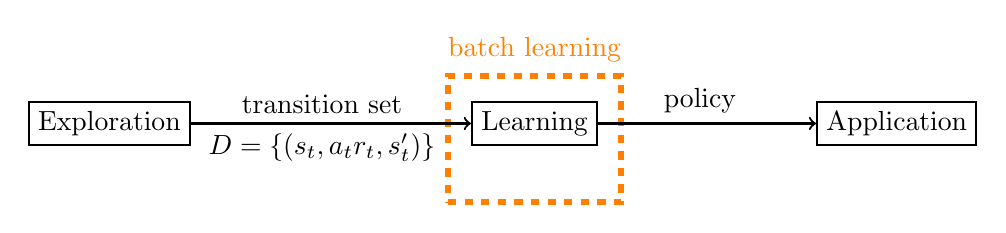
\begin{tikzpicture}[node distance = 16em, auto, thick]
    \node[draw] at (0, 0)   (A) {Exploration};
    \node[draw] at (5.4, 0)   (B) {Learning};
    \node[draw] at (10, 0)   (C) {Application};
    \draw[orange, dashed, line width=0.7mm] (5.4,-0.2) node[minimum height=1.6cm,minimum width=2.2cm,draw, label={above: batch learning}] {} ;
    
    \draw[->] (A) node[above, xshift=2.7cm] {transition set}  node[below, xshift=2.7cm] {$D = \{ (s_t, a_t r_t, s'_t)  \}$} -- (B);

    \draw[->] (B) node[above, xshift=2.1cm] {policy}  -- (C);
\end{tikzpicture}
	\caption{Batch Reinforcement Learning}
	\label{fig:batchlearning}
\end{figure}

Because exploration has an important impact on the achieved policy quality, more modern \emph{growing batch reinforcement learning} approaches frequently alternate between exploration and learning phase as shown in \Cref{fig:growingbatchlearning}. In doing so, the agent gets a rough idea of a good policy in order to focus on \emph{interesting} regions of the state space.

\begin{figure}[ht]
	\centering
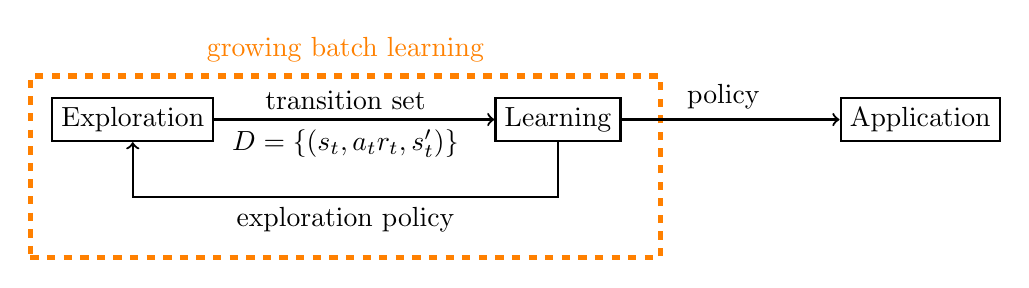
\begin{tikzpicture}[node distance = 16em, auto, thick]
    \node[draw] at (0, 0)   (A) {Exploration};
    \node[draw] at (5.4, 0)   (B) {Learning};
    \node[draw] at (10, 0)   (C) {Application};
    \draw[orange, dashed, line width=0.7mm] (2.7,-0.6) node[minimum height=2.3cm,minimum width=8cm,draw, label={above: growing batch learning}] {} ;
    
    \draw[->] (A) node[above, xshift=2.7cm] {transition set}  node[below, xshift=2.7cm] {$D = \{ (s_t, a_t r_t, s'_t)  \}$} -- (B);
    \draw[->] (B.south) node[below, xshift=-2.7cm, yshift=-0.7cm] {exploration policy}  -- ++(-0,0) -- ++(0,-0.7) -| (A);
    \draw[->] (B) node[above, xshift=2.1cm] {policy}  -- (C);
\end{tikzpicture}
	\caption{Growing Batch Reinforcement Learning}
	\label{fig:growingbatchlearning}
\end{figure}

\subsection{Tree-Based Batch Mode Reinforcement Learning}
Randomized decision trees can be used to approximate the parameters of $Q(s, a; \theta)$, as proposed by Damien Ernst \Cite{Ernst:2005:TreeBasedBatchModeRL}. The batch reinforcement learning algorithm is shown in \Cref{alg:fittedQiteration}.\\

\begin{algorithm}[H] 
 \caption{Fitted Q Iteration \Cite{Ernst:2005:TreeBasedBatchModeRL}.}
     \SetAlgoLined
          \footnotesize
     
     \KwIn{$D=\{  (x_t, a_t, s_t, r_t), \dots{} | t=1..n  \}$}

     $\hat{Q} \leftarrow 0$\;
     $k \leftarrow 0$\;
     \Repeat{stopping condition reached}{
     $k \leftarrow k + 1$\;
      generate pattern set $P = \{(i^t, o^t) | t=1,.., n\}$ where\;
      \Indp    $i^t = (x^t, a^t),$ \hspace{0.7cm}  $o^t = r_t + \gamma * \max\limits_{u} \hat{Q}^k(s_t, u)$\;
      \Indm $\hat{Q}^{k+1} \leftarrow ^{fit} P$
     }
\label{alg:fittedQiteration}
\end{algorithm}\bigskip


\section{Optimized Trade Execution}
As outlined in \Cref{chap:objectives}, the problem of \emph{optimized trade execution} is defined by a particular financial instrument, which must be bought or sold within a fixed time horizon, while minimizing the expenditure (share price) for doing so. In order to achieve the best possible price, proper timing is crucial to reduce hidden costs like slippage (see \Cref{chap:slippage}).\\

The general task of this thesis is to apply reinforcement learning to successfully learn state-based strategies for optimal order placements. Based on the observed market situation and trade progress the obtained \acl{SR} (see \Cref{chap:tradingstrategies}) may become more or less aggressive as time passes.\\

The examined agents derive their strategies from a (growing) batch of sample transitions stemming from interactions with a simulated trading environment, that is described in the next chapter.




\cleardoublepage{}